\chapter{Templates}

Regular users can create/modify Personal Templates.
However, the Administrator has to grant special permissions for a regular user to create/modify Global Templates.

\section{Global Templates}
Obidos comes with a number of predefined Global Templates. These Global Templates are available to all users.

\section{Personal Templates}
A Personal Template belongs to an individual user and not available/visible to other users.
A user can create a Personal Template from scratch or create one by cloning a Global Template.

\section{Templates Management}
Other than the visibility, Creation/Modification of Global Templates and Personal Templates are done the same way.
\subsection{Creating a Template}

To create a new Personal Template, select "Create new Personal Template" from the top level Templates menu on the Main Menu bar (see the following Figure).

\begin{figure}[H]
\centering
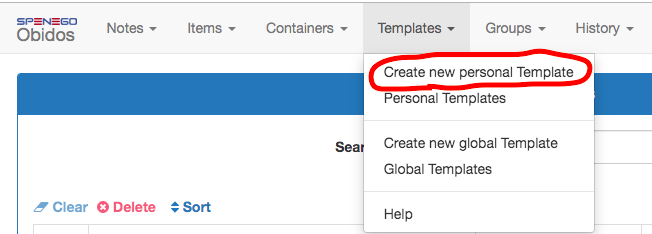
\includegraphics[scale=0.4]{user/Create-Personal-Template-Menu.png}
\caption{Create new Personal Template}
\label{fig: Figure}
\end{figure}

The following figure shows the screen for creation of the Personal Template.

\begin{figure}[H]
\centering
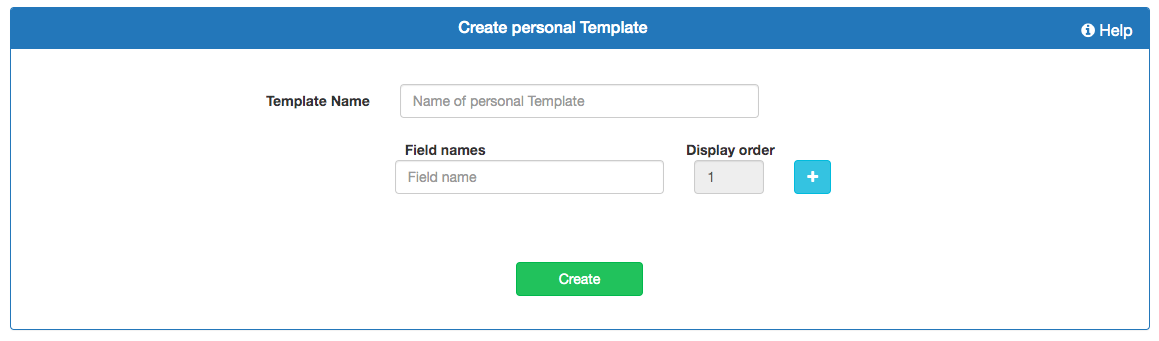
\includegraphics[scale=0.4]{user/Create-Personal-Template-Screen-1.png}
\caption{Screen for new Personal Template}
\label{fig: Figure}
\end{figure}

The name of the Template is used in the listings and searches. It can be upto 64 characters long.
A field name can be upto 32 characters long. The "Display order" decides the order in which the fields
will be displayed from top to bottom. To add a new field, click on the 
{\color{myblue}\faPlusSquare} button. Adding a second field will display a screen as shown in the following Figure.

\begin{figure}[H]
\centering
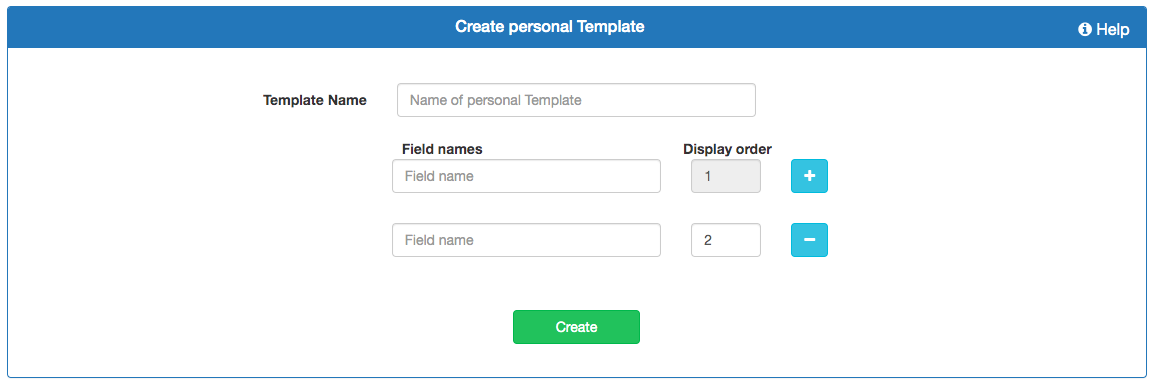
\includegraphics[scale=0.4]{user/Create-Personal-Template-Screen-2.png}
\caption{Adding fields to a Template}
\label{fig: Figure}
\end{figure}

To remove a field, click on the {\color{myblue}\faMinusSquare} button.

\subsection{Creating an Item Using a Template}
Consider a Template named testTemplate with 5 fields as seen in the following Figure.

\begin{figure}[H]
\centering
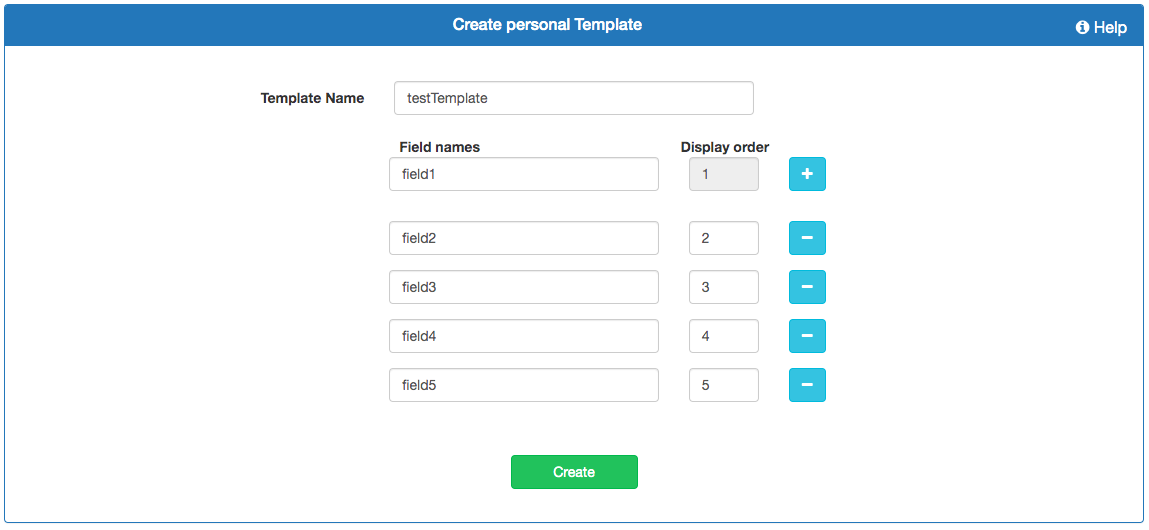
\includegraphics[scale=0.4]{user/Personal-Template.png}
\caption{Personal Template with 5 fields}
\label{fig: Figure}
\end{figure}

When testTemplate is used to create an Item, the screen will present like this:

\begin{figure}[H]
\centering
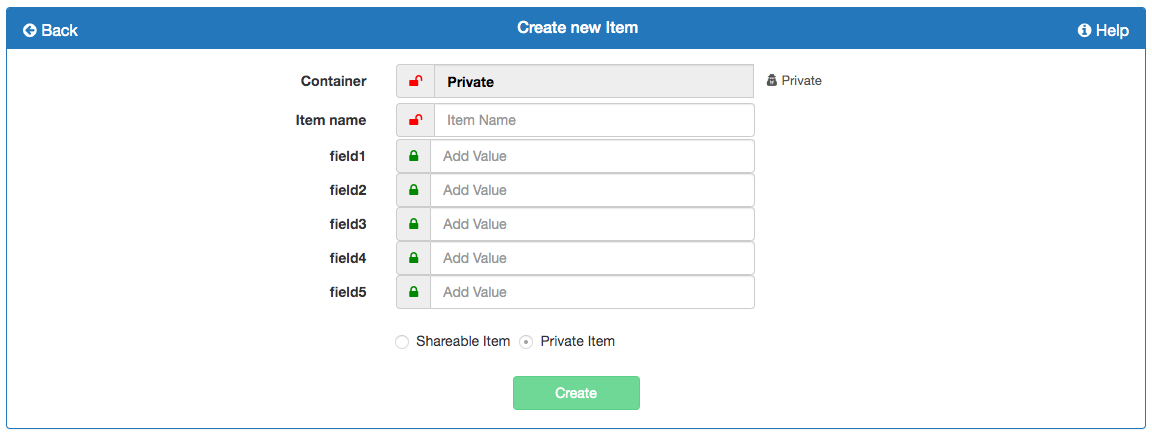
\includegraphics[scale=0.4]{user/Create-Item-With-Personal-Template.png}
\caption{Creating an Item using testTemplate}
\label{fig: Figure}
\end{figure}

